\section{Reducing Overheads of Run-Time Monitoring}
\label{sec:optimizations}

% Overview of overhead vs. coverage space
\begin{figure}
  \begin{center}
    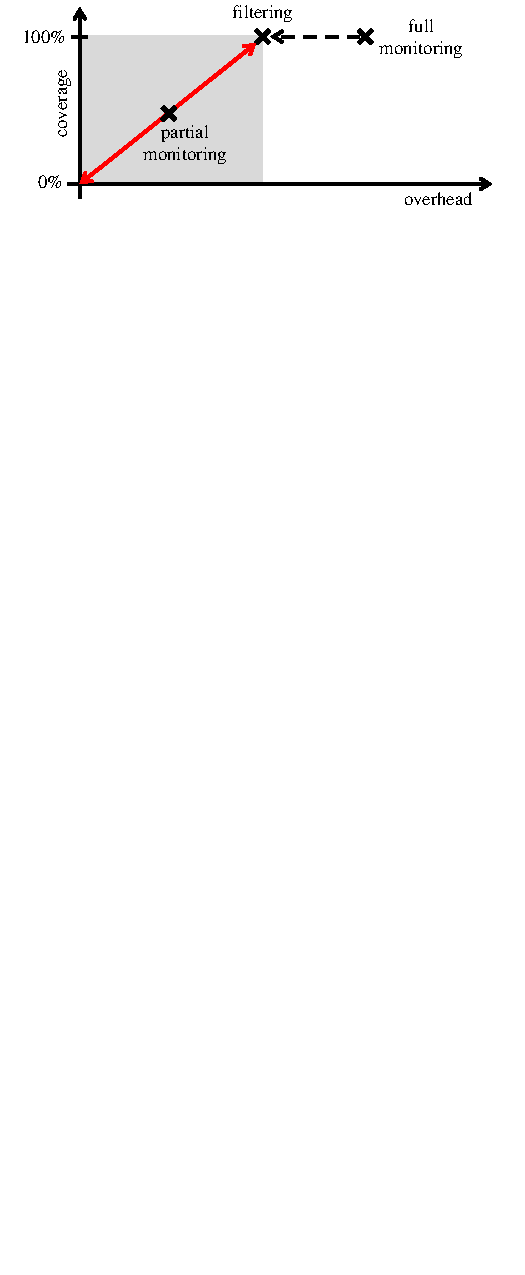
\includegraphics[width=\columnwidth]{figs/optimization_overview.pdf}
    \vspace{-0.2in}
    \caption{Filtering can be used to reduce the overheads. Partial monitoring
    allows a further trade-off between coverage and overheads.}
    \label{fig:optimizations.overview}
    \vspace{-0.1in}
  \end{center}
\end{figure}

Although the monitoring core operates in parallel to the main core, the
overheads of programmable monitoring can be high due to the multi-cycle
operation of the monitoring core.
Figure~\ref{dummy} shows the full
monitoring overheads for three example monitoring extensions: array bounds
check (BC), uninitialized memory check (UMC), and dynamic information flow
tracking (DIFT) (Section~\ref{sec:evaluation} details the experimental methodology). In order to reduce these overheads, we present two
optimizations. The first optimization is to filter out monitoring events which relate to
null metadata which do not need to processed by the monitoring core (Section~\ref{sec:optimizations.filter}). Second, in order to allow
further reduction in overheads, we propose to perform partial monitoring. This
allows us to further reduce the overheads of monitoring by trading-off
monitoring coverage. Figure~\ref{fig:optimizations.overview} shows an overview
of
these ideas.

\subsection{Filtering Null Metadata Events}
\label{sec:optimizations.filter}

The instruction-grained run-time monitoring schemes we focus on typically
manage a set of metadata information. This metadata information is used to
verify security or reliability properties. For example, for array bounds
check, the monitoring core stores metadata describing the base and bound
addresses for array pointers. This metadata is then checked on load and store
instructions. However, if the metadata for an event is null, then there is no
need to perform the check since this represents a non-array pointer value. By
identifying and filtering out these null monitoring events, we can reduce the
overheads of
monitoring by reducing the amount of work the monitoring core must do.

In order to filter out null monitoring events, we need an efficient method to
keep track of which events are null. In addition, when we filter out a null
monitoring event, we must ensure that any metadata propagations that were
skipped are handled properly. If this is not done, the monitoring core may
operate on stale metadata. Thus, when we filter out a null monitoring event,
we must ensure that the destination metadata is also marked as null. 
In other words, we need to be able to track not only
metadata which is initially null, but also the dataflow of null metadata. 

\subsection{Trading-Off Coverage for Reduced Overheads}
\label{sec:optimizations.drop}

There is a limit to the reduction in overheads that can be achieved by using
filtering alone. We propose to further reduce overheads
by performing partial monitoring. As the
monitoring schemes we target consist of a large number of independent
monitoring checks, it can still be possible to provide partial protection by
performing a portion of the monitoring operations. Thus, we aim to enable this
trade-off between overheads and monitoring coverage.

Our goal in using partial monitoring is to allow the user or system designer to
specify their acceptable overheads. Given this overhead budget, monitoring is
only performed as long as this budget is not exceeded. If the overhead budget
is exceeded, then monitoring operations are dropped. This creates an adjustable
trade-off between the overheads incurred and the monitoring coverage achieved.

Dropping monitoring operations implies that some functionality of the
monitoring scheme has been lost.  This may cause either false negatives, where
an error that occurs in the main program's execution is not detected, or false
positives, where the monitor incorrectly believes an error has occurred.  For
example, a false positive can occur for array bounds check if an event is
dropped that handles copying a pointer. Since the new pointer does not have
correct base and bound address metadata, it will incorrectly cause errors to be
raised.  We accept false negatives as the
loss in coverage that we trade off in order to limit overheads.  However, we
must safely drop monitoring events in such a way as to avoid false positives so
that the system does not incorrectly raise an error.

In analyzing various monitoring schemes, we found that monitoring operations
are primarily of two types: \emph{checks} and \emph{metadata updates}. Monitors
\emph{check} certain properties to ensure correct main program execution and
they \emph{update} metadata for bookkeeping. Skipping a check operation can
only cause false negatives and will never cause a false positive. Therefore, we
may simply skip a check operation. Skipping an update operation can cause false
negatives but may also cause false positives. Essentially, when an update
operation is skipped, we can no longer trust the corresponding metadata. Thus,
we need to be able to mark these invalid metadata. Furthermore, metadata that
would be derived from these dropped events also will be invalid. In other
words, we need to be able to track the dataflow of invalid metadata when
monitoring operations are dropped.
